\chapter{Survivability of Hierarchical Networks}
\label{chapter.SurvivabilityOfHierchicalNetworks}
\markright{Survivability of Hierarchical Networks}

\section{Background}
Recent developments in transport networks have resulted in an increasing
concentration of high capacity traffic on fewer network elements.
Hence, the risk of losing large amounts of data becomes imminent and
maintaining a high level of network survivability becomes desirable.
Network survivability relates to the ability of a network to recover
from network element failures. Typically, service providers (or carriers)
provision backup or redundant network resources to protect their services
against network failures. However, they are equally faced with the
objective to efficiently utilize their network resources.

Several factors are considered when designing survivability options
in transport networks. The most important are: resource utilization,
connection request blocking, restoration recovery time, recovery ratio,
recovery granularity, control complexity, tolerance of single or multiple
faults and scalability; the goal being ideally to achieve maximum
survivability with minimum recovery time, while maintaining maximum
resource utilization. It is hard to achieve all these goals simultaneously,
so trade-offs are typically considered when designing a realistic survivable
network. For example, dedicated protection schemes usually offer faster
recovery than restoration schemes; however, they are less resource-efficient.


\section{Protection and Restoration Schemes}

Throughout the literature the terms protection and restoration are
used in slightly different meanings. Protection makes use of pre-assigned
capacity between nodes. This includes the pre-calculation of the protection
path and the preplanning of resources. To provide protection of a
working connection, guaranteed recovery with similar grade of service
and sufficient amount of bandwidth must be set aside in the network.

Depending on the different time-scales in which the spare capacity
is allocated, there are essentially two types of fault management
techniques: protection and restoration. Prior to performing recovery,
the layer closest to the failure is responsible for detecting the
failure. Network nodes communicate with each other to determine where
the failure has occurred and notify other network elements of the
failure. Depending on the different time-scales in which the spare
capacity is allocated, there are essentially two types of fault management
techniques: protection and restoration.

In restoration, signaling is used in real time after the failure occurs
to reroute traffic onto newly computed paths. The LSP is able to compute
the route of the backup LSP according to the automatically updated
routing table after the failures happen. The main disadvantage of
this scheme is its recovery time, mainly due to its dependency on
the slow convergence of IP routing protocols. The advantage of this
scheme is its ability to react to complicated scenarios such as multiple
simultaneous failures.

In protection, however, backup paths are pre-provisioned, and spare
capacity is reserved for them at the time the working path is set
up. Protection techniques can be implemented by several architectures
(for example, 1+1, 1:1, 1:N, and M:N).

Generally, protection is more resource costly, since it requires pre-allocation
of spare capacity for the pre-established backup paths. On the other
hand, restoration may take longer to restore the connection, since
the restoration process happens in real-time. Protection and restoration
have traditionally been addressed using two techniques: end-to-end
path switching and local span/link switching.

Protection and restoration have traditionally been addressed using two techniques: end-to-end path switching and local link switching [XXX].

\begin{figure}
\centering 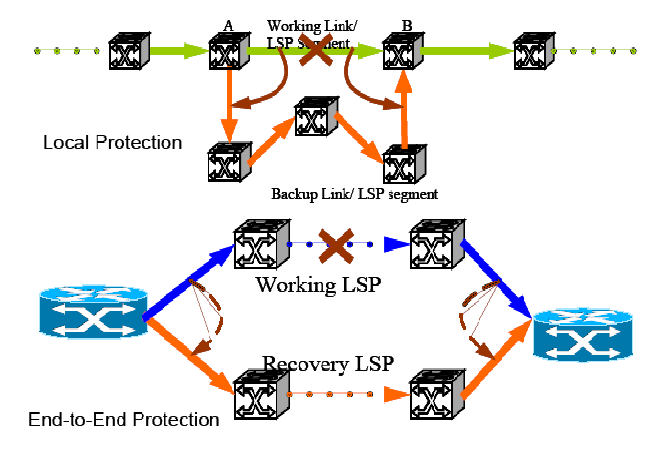
\includegraphics[scale=0.75]{Figures/LocalVsE2EProtection}
\caption{Local versus end-to-end LSP protection}
\label{fig:LocalVsE2EProtection} 
\end{figure}



\subsection{Local versus End-to-End Recovery}
End-to-end recovery refers to the recovery of an entire LSP from its
source (ingress router end-point) to its destination (egress router
end-point). Local/segment recovery refers to the recovery over a portion
of an LSP segment. Figure~\ref{fig:LocalVsE2EProtection} depicts
the difference between local and end-to-end protection.

In an end-to-end path protection scenarios {[}7, 8], a preestablished
backup LSP is set up from ingress label switched router (LSR) to the
egress LSR. In order to guarantee maximum availability, the backup
LSP path is typically routed over a physically disjoint path from
the working LSP. When the ingress LSR is notified of failure on the
working LSP (e.g., reception of a signaling RSVP Path Error due to
the failure of a network component), the ingress LSR immediately starts
switching traffic over to the backup LSP.

In normal situations, the backup LSP does not normally carry any protected
traffic as long any resources along the working LSP have not failed.
For efficiency, and to make best available use of network resources,
it is common practice to allow backup paths to carry traffic (referred
to as low-priority traffic or extra traffic). This low-priority traffic
gets preempted by the high-priority protected traffic when the working
LSP fails.

A similar approach to path protection can be implemented on a link
switching-- also referred to as local link protection. A backup LSP
only spans a link (or a node) to protect this link (or node) {[}FRR].
The backup LSP originates at the protection switch LSR-- also known
as the Point of Local Repair (PLR)-- and terminates in the protection
merge LSR or Merge Point (MP) where the backup LSP is merged with
the working LSP. It is important to note that if a working LSP spans
several links, one backup LSP has to be set up for each protected
link along the working LSP path in order to protect the entire working
LSP.

Path protection reacts to failures more slowly than local protection,
since it takes a significant amount of time to notify the ingress
LSR to switch over to the backup LSP. This leads to more packet loss.
On the other hand, only one backup LSP is needed for one working LSP,
and its global nature allows for less spare resource requirements.

A hybrid scheme named referred to as Fast Reroute was also proposed
FRR. A backup LSP is provided in the opposite direction and concatenated
to a physically disjoint LSP. It combines the best characteristics
of both path and local protection schemes; see {[}9] for more detail.


\subsection{1+1 Protection}

The 1+1 protection scheme refers to the case where one dedicated protection
LSP protects exactly one working LSP or link and protected traffic
is permanently duplicated at the ingress node on both the working
and protection LSPs. Both the primary and backup paths are set up
at the same time, and the required bandwidth is allocated for both.
Upon failure, the destination node can select, independently from
the source node-- \emph{e.g.}, by monitoring the signal quality or
Bit Error Rate (BER)-- the preferred LSP to receive protected traffic
on. Upon failure, the destination can switch (i.e., non-signalled
switchover based on LOS, etc.) from one LSP to another. Hence, $1+1$
protection implicates no signaling delays after failure. Although
such recovery is very fast, it is also inefficient due to the inherent
resource redundancy dictates that extra traffic can be carried over
the protection LSP while the primary or working LSP is active.


\subsection{1:1 and 1:N Protection}

The 1:1 (\emph{aka}, $1-to-1$) protection scheme refers to the case
where one specific backup LSP protects exactly one specific working
LSP/span but the normal traffic is transmitted over only one LSP/span
(working or protecting) at a time. Both working and protection paths
are provisioned simultaneously, but data is only forwarded over the
working path. As a result, protection paths can be used to transmit
low priority pre-emptable traffic during non-failure conditions. As
in 1+1 protection, failure recovery is relatively fast, but efficiency
is somewhat improved.

The 1:N (\emph{aka} $n-to-1$) protection is a extension case of the
1:1 protection. The basic idea of 1:N protection, is that one backup
LSP can protect N working LSPs/spans. When provisioning the working
path, the backup path is negotiated but the allocated bandwidth can
also be used for low-priority traffic (extra-traffic).


\subsection{Shared Mesh Restoration and N:M Path Protection}

Shared path protection builds upon the advantages of 1:N by further
increasing resource efficiency. The backup resources, in this case,
can be shared amongst many LSPs if they fail independently. Since
resources along the protection path are shared, switch nodes along
the protection path are not configured at connection setup. Instead,
upon a failure, source nodes (of failed paths) are notified and generate
signaling messages to configure the switches along the protection
path.

Path-based protection schemes such as 1:1 or n:1 consider the protection
of service traffic between two particular nodes. For path-based schemes,
arrival of a request to establish shared mesh protection service between
two nodes can prompt computation of a pair of disjoint connections
between them. The primary and protection connections would be set
up, meeting the following two necessary requirements.

First, sufficient bandwidth should be available along the route of
the working connection to accommodate the requested load. Second,
either of the following two conditions must hold: either whatever
bandwidth for protection had previously been reserved along the protection
path is already sufficient to guarantee recovery from any single link
or node failure along the new working path, or there must be enough
available bandwidth along the protection path to accommodate the additional
reservation. From the point of view of the network, the degree to
which the additional bandwidth for protection should be shared in
this manner depends on the failure coverage objective for the particular
LSP: whether the objective for the LSP is protection against failure
of any single node, of any single link, or of an SRG.

TODO: FIXME Both shared mesh restoration as well as the N:M path protection
offer sharing for protection resources for multiple working LSPs.
Specifically, in the N:M protection case, N multiple backup LSPs can
potentially protect M working LSP/spans. Backup LSPs .

Shared-mesh restoration, on the other hand, is defined as a particular case of pre-planned LSP re-routing that reduces
the restoration resource requirements by allowing multiple restoration
LSPs (initiated from distinct ingress nodes) to share common resources
(including links and nodes).

%
\begin{figure}
\centering 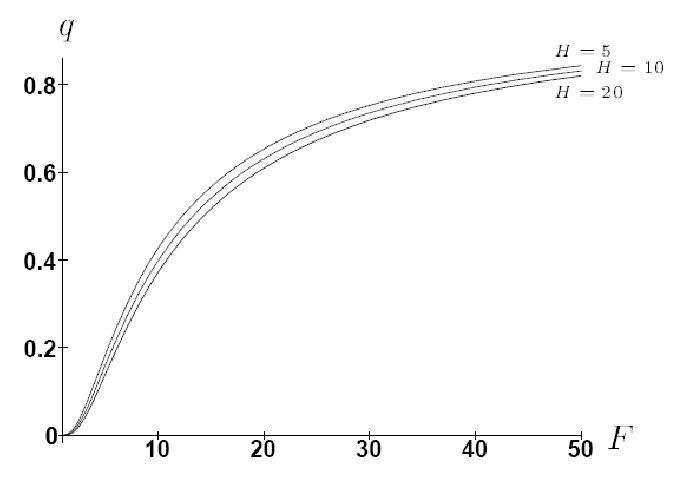
\includegraphics[clip]{Figures/util1} 

\caption{Blocking probability for different path hops \emph{H}}


\label{fig:Utilization} 
\end{figure}



\section{Survivability in Hierarchical Networks}

Transport networks are planned to recover from failures due to a risk
using different mechanisms at different layers. Establishing a primary
path disjoint from the secondary reduces the chances of losing or
dropping traffic for longer time. Indeed, it is imperative to note
that path disjointness at one layer does not necessarily infer physical
path disjointness at all lower layers.

As described earlier, transport networks are structured in vertical
and horizontal structure. This motivates the need to study survivability
of a connection crossing vertical as well as horizontal layers of
the transport network.


\subsection{Survivability across Vertical Layers}

GMPLS networks can be segmented into several areas, such as, wavelength,
waveband, and fiber areas in order to optimize the resilience and
scalability of the networks as shown in Figure 3.1. The achievable
availability of a connection depends highly on the proper identification
and selection of a protection layer. The protection layer is defined
with the following two characteristics: (1) it is one of those layers
below the layer containing the connection; and, (2) the connection
will be protected against resource failures in the protection layer
{[}PIC06].


\subsubsection{Recovery at highest layer}

With recovery at highest layer, the traffic is recovered at the layer
where the traffic is injected. This recovery approach allows the provision
of different survivability classes at a high granularity. On the other
hand, in case of physical failures like cable cuts, a large number
of connections must be recovered individually. This results in a slower
recover performance, as we will attempt to show with simulation results.
With recovery at the highest layer the single layer recovery mechanisms
need not be coordinated, since the mechanisms in the different layers
work independent of each other. At the planning phase of the network
it must however be assured, that client demands of working and protection
network connections are not protected within the server (lower) layer.


\subsubsection{Recovery at lowest layer}

When using recovery at the lowest layer disrupted traffic is restored
at the layer closest to the failure. If a network has to be 100\%
protected against all single link and single node failures, spare
resources in the client layer are only needed for multi-hop client
connections. Due to fault propagation, the client layer detects failures
caused by server layer or physical layer failures. It must be stressed
that the client layer in some cases cannot distinguish whether defect
detection is due to a failure at the client layer itself, or due to
a failure at the server layer. Hence, recovery mechanisms must be
coordinated to prevent a contention between them. Three such interworking
strategies are presented next.


\paragraph{Uncoordinated Recovery.}

In the uncoordinated recovery no interworking mechanism is used to
coordinate the recovery mechanisms. The client layer switches an affected
connection to a backup path as soon as a defect is detected. However,
if the failure occurred in the physical layer, the server layer also
starts the recovery. Due to a time delay between the detection of
failures and the completion of the recovery mechanisms, it may happen
that failures which were already recovered by the lower layer are
again switched to another recovery path in the client layer. This
second switching causes a secondary temporary disruption of already
recovered connections and client layer spare resources will be unnecessarily
occupied. If low priority traffic was carried as extra traffic on
these spare resources, this traffic is unnecessarily pre-empted, causing
additional loss of (low priority) traffic.


\paragraph{Hold-off Time.}

The drawbacks of an uncoordinated recovery prove the need for an interworking
strategy for the coordination of the recovery mechanisms. A simple
and robust interworking strategy is the adoption of a hold-off time
to delay the activation of a higher layer recovery mechanism. The
hold-off time has to be dimensioned large enough so that the lower
layer recovery has enough time to finish the recovery process. If
after the elapse of the hold-off time the upper layer connections
are still affected by the failure, the higher layer recovery will
be activated. The advantage of this solution is its simplicity and
robustness. The obvious drawback is that in some failure scenarios
the higher layer recovery is delayed even if the lower layer recovery
is not able to recover the failure.


\paragraph{Recovery Token.}

To improve the recovery performance in situations where the lower
layer recovery fails, a recovery token delivered to higher layer and
trigger recovery may be employed.


\subsection{Survivability across horizontal layers}

In addition to being vertically layered, optical transport networks
may consist of multiple domains since different carriers or service
providers may want to manage their own parts of the network similar
to the Internet that is formed of great number interconnected Autonomous
Systems (ASes). In this case, a horizontal hierarchical representation
of the network topology can be applied to achieve better scalability.
In this situation, a global connection is likely to cross multiple
domains before it reaches its destination. Connections between regions
or domains can be maintained as abstract (or logical) links. This
process typically includes three main components: an aggregation scheme,
an update policy and a routing algorithm. In Chapter XX, we define
an aggregation scheme that is suitable for calculation of diverse
path at the domain level as well.

We distinguish between inter- and intra- protection techniques for
networks that are separated into several areas. The nodes interconnecting
two or more areas are called border nodes. Intra-area protection implies
that a failure can be restored within the affected areas. This is
done either by local area protection (i.e., by the node adjacent to
the failure) or by the border node on the path to the source. Hence,
local protection is more efficient and faster than end-to-end path
protection across the whole network. Inter-area protection implies
that a connection can be protected against a whole domain failure
and that a connection can be restored by through a path that reroutes
around the failure domain.


\section{Survivability of QoS-sensitive Traffic}

The Internet carries a variety of applications that have varying requirements
for network reliability. For example, some applications, such as email,
do not need the same high reliability as real-time medical or banking
information. Also, it is not cost-efficient to provide equal resilience
to all different type of traffics running over the Internet. Thus,
it would be more realistic to provide differing levels of network
survivability to various traffic types in accordance with the respective
Service Level Agreement (SLA) and try to maximize the network utilization
{[}IWA00].

While the standard routing protocols based on Constraint-based Shortest
Path First (CSPF) algorithms are suitable for establishing new LSPs,
they are too slow to be used for dynamic rerouting of QoS-sensitive
traffic in the presence of node and link failures. In SONET-based
networks bandwidth restoration and protection occurs at the SONET
level. However, where SONET-based restoration is not available, other
protection mechanisms become necessary to ensure that bandwidth guarantees
are still in place upon link or node failure; example of the new emerging
technology that suitable for non-SONET level is Bidirectional Fault
Detection (BFD) Mechanism.


\section{Path Diversity and SRLGs}

One important requirement of survivable network design is the ability
to discover diverse routes for client connections. Multiple connections
are often setup between endpoints for primary and backup paths with
a constraint of being diversely routed. This can include paths that
are link-diverse (i.e. do not share any common link), or node-diverse
(i.e. which do not share any node). This characteristic of path computation
can become complicated when multiple layers (physical and logical)
are considered.

Finding diverse protection paths in a layer in a multilayered network
is a challenging problem. For example, in a hierarchical optical network
an MPLS packet LSP is tunneled inside a lambda-LSP tunneled inside
a fiber-LSP. Multiple fibers are placed into conduits, which are buried
along the right of way (ROW). For economic reasons, service providers
rent ROWs from third parties, such as the railroad companies. As a
result, two diverse fiber links at the OXC layer may be placed into
the same conduit at the conduit layer and are subject to a single
point of failure. Such links cannot be regarded as diverse links when
being used to compute working and protection path pairs. Shared risk
link group (SRLG) was proposed to address this problem {[}XU 03]and
{[}XU 04]. An SRLG is a group of links that are subject to a common
risk. The SRLG concept can be applied to physical as well as logical
resources at all layers of the network

Therefore, finding a pair of diverse paths at the optical layer involves
computing a pair of SRLG-diverse paths. Although the concept of SRLG
was originally proposed to deal with conduit cuts, it can be extended
to include general risks. For example, all the fiber links located
in a geographic area may be assigned the same SRLG considering the
risk of earthquakes. In our study an SRLG risk in this paper represents
a general risk.


\section{Service Availability}

Service availability between two nodes in a network refers to the
ability of the network to perform its primary function (e.g., IP packet
forwarding). This involves physical connectivity, link-layer protocol
connectivity, and network-layer protocol connectivity. Today's ISPs
offer their customers a guarantee of port availability as part of
their SLAs. This simply represents the uptime of a single network
element, i.e., the hardware by which the customer attaches to the
ISP's network. However, this does not, in any way, provide guarantees
about the destinations that a customer can reach at a given point
in time. A key requirement for service availability between two nodes
is the existence of physical connectivity between the nodes (path
availability). A link failure that impacts path availability will
also impact service availability.

It is desirable sometimes to guarantee survivability on per connection
basis, since this provides a means to measure its survivability in
a quantifiable manner. The pre-defined approach to handling LSP protection,
such as letting the high-priority LSPs use optical-layer protection
and the lower-priority LSPs use IP-layer protection, is at times not
sufficient. This is because customer usually demands a more concrete
threshold for guaranteed services. In this case, the connection survivability
guarantee can be specified in terms of minimum connection availability,
defined as the fraction of time the service is available between both
ends of a connection. Several equations describe the basic concepts
that define availability:

\begin{equation}
Availability=1-\dfrac{(Total\ connection\ outagetime)}{(Total\ in\-service\ connection\ time)}
\end{equation}


Availability for devices can be expressed as the following equation
for mean time between failure (MTBF) and mean time to repair (MTTR):

\begin{equation}
Availability=\dfrac{MTBF}{(MTBF+MTTR)}
\end{equation}


The classic availability objective for the public switched telephone
network (PSTN) is to provide 99.99\% availability. Thus, a definition
of service availability in a multilayered network typically considers
the following factors: 

\begin{itemize}
\item network topology, 
\item mapping of IP links onto the underlying physical infrastructure, 
\item inter-dependence of IP network elements, 
\item failure characteristics of links/routers, and 
\item routing protocol convergence time. 
\end{itemize}

\subsection{Hierachical Link Availability}
The availability of a higher layer link (e.g., IP link) depends on
the underlying link layer protection. For example, for a (1+1) protection
scheme at lambda layer, assuming $F_{1}$ the set of fibers that are
crossed by the primary lightpath at the optical layer, and $F_{2}$
the set of fibers crossed along the backup lightpath, the IP link
will fail only when both the primary and the backup lightpaths fail
simultaneously. The availability $A_{l}$ of link $L$ in this case
can be written as:

\begin{equation}
A_{l}(L_{1},L_{2},1+1)=
	\prod_{f\in F_{1}}A_{f}+\prod_{f\in F_{2}}A_{f}-\prod_{f\in F_{1}\cup F_{2}}A_{f}
\label{eqn:1Plus1Availability}
\end{equation}


For a link at a higher layer that is using shared protection (e.g.
1:N) protection, the link will fail if: 

\begin{itemize}
\item both the primary and the backup lightpaths fail, or
\item the backup does not fail but the primary and at least one other lightpath that share the same backup fail at the same time. 
\end{itemize}

Let $F_{b}$ be a set of fibers in other lightpaths that share the same backup lightpath. The availability of a 1:N protected link in this case can be written as:

\begin{equation}
A_{l}(L_{1},L_{2},1:N)=\prod_{f\in F_{1}}A_{f}+\prod_{f\in F_{2}\cup F_{b}}A_{f}-\prod_{f\in F_{1}\cup F_{2}\cup F_{b}}A_{f}
\label{eqn:1For1Availability}
\end{equation}



\subsection{Hierarchical LSP Availability}
Assuming an LSP at a certain network layer $m$ traverses a subset
$L_{u}nprot$ of unprotected links at a lower layer, a subset $L_{1+1}$
of 1+1 protected links at layer $m-1$, and a subset $L_{1:N}$ of
1:N protected links at layer $m-1$, the availability of that LSP
is therefore:

\begin{equation}
A_{LSP}=\prod_{f\in L_{unprot}}A_{l}\bullet\prod_{f\in L_{1+1}}A_{l}\bullet\prod_{f\in L_{1:N}}A_{l}
\label{eqn:LspAvailability}
\end{equation}


The availability of an inter-domain LSP that traverses multiple domains
offering different protection types for each portion of the LSP crossing
the domain:

\begin{equation}
A_{inter-LSP}=\prod_{d=1}^{n}A_{LSP}^{d}-\prod_{d\in d_{1}\cup d_{2}\cdots d_{n}}^{n}A_{LSP}^{d}
\label{eqn:InterLspAvailability}
\end{equation}

\section{Analysis of LSP Blocking Probability}
For the purpose of evaluation of network performance and optimization for different proposed techniques, it is typical to define an objective function. As a natural choice the total \emph{network revenue} can be considered. According to this approach, LSP requests accepted on a certain path $r$ generate revenue at a rate $w_r$, and the total expected network revenue is then:

\begin{equation}
W=\sum_r w_r\lambda_r = \sum_r w_r \nu_r(1 - B_r)
\end{equation}

where $\lambda_r$ is the carried traffic on route $r$, $v_r$ is the traffic offered to path $r$ and $B_r$ is the end-to-end blocking probability for path $r$.

If $w_r$ is proportional to the bandwidth requirement of each LSP request then $W$ signifies the total carried traffic in the network.

Consider a network with $J$ links connected in an arbitrary topology. Denote $C_j$ for the number of circuits in link $j$. At a given instant of time, some of the bandwidth (circuits) on link $j$ will be allocated while the remainder free. Let $m_j$ denote the number of idle circuits on link $j$ , and let $\textbf{m} = \{m_1, \cdots , m_J\}$ denote the network state. The state space is given by $\Lambda = \{0, \cdots, C\} \times \cdots \times \{0, \cdots , C_J\}$.

A path $R$ is a subset of links from ${1,2, \cdots, J}$. Denote $R_j$ for the set of paths that employ link $j$. In order for a LSP call to be set up on path $R$, at least k-units of requested bandwidth must be available at each link $j \in R$. Denote the rate at which LSP calls requests are \emph{set up} path $R$ when the network is in state $m$ by $\lambda_R(m)$. In this case, $\lambda_R(m)$ satisfies:

\begin{equation}
\lambda_R(\textbf{m})= 0 \text{ if } m_j=0 \text{ for some } j \in R.
\end{equation}

Consider the situation where LSP requests arrive to path $R$ at rate $a_R$ and an LSP request is setup on path $R$ if and only if $mj > 0$ for all $j \in R$. Thus,

\begin{equation}
\lambda_R(\textbf{m})=
\begin{cases}
a_R, &\text{if $m_j > 0~\forall j \in R$.} \\
0, &\text{otherwise}
\end{cases}
\end{equation}


\subsection{Unprotected LSP Blocking}
Consider the situation where an ingress LSR attempts to signal an LSP from source $s$ to destination $d$ over a path with $n$ hops. Assuming that an LSP request will be established if at least 1-unit of bandwidth is available on each link, and each link has a capacity of $C$ units of bandwidth.

Let $p$ be the probability that a link $L$ along the path of the LSP is busy (i.e. at least 1 unit of bandwidth is in-use). The expected bandwidth allocation on $L$ can be writtend as $\rho \bullet C$, and $\rho$ in this case signifies the utilization of Link $L$ on this path. An LSP from $s$ to $d$ is blocked if at least one of the links along the path has reached its full capacity (\ie\ fully utilized).

The probability that the LSP request is \emph{blocked} at any link $j$ is:
\begin{equation}
P_b^j = \left( \rho_j \right) ^C
\end{equation}

and the probability the LSP is \emph{admitted} at link $j$:
\begin{equation}
\begin{split}
P_a^j &= 1 - P_b^{j} \\
	  	&= 1 - \left( \rho_{j}\right) ^{C}
\end{split}
\end{equation}

Assuming all links have the same capacity $C$, the probability $P_B^L$ that an LSP request crossing $N$ hops gets blocked can be written as:
\begin{equation}
P_b^L(s,d) = 1-\prod_{n=1}^{N} P_{a}^j
\end{equation}

Rearranging, define the achievable utilization for a given blocking probability as:
\begin{equation}
q=\left[ 1 - (1 - P_b)^{1/N} \right]^{1/C}
\end{equation}	

and for small $\frac{P_b}{N}$, $q$ can be written as: 
\begin{equation}
q \simeq \left( \dfrac{P_b}{N} \right)^{1/C}
\end{equation}

\subsection{Path-protected LSP Blocking}
Considering the case of a 1+1 path-protected tunnel, for the LSP request not to be blocked, both the working and backup paths have to checked and reserved. The probability $P_b(1+1)$ that the request gets blocked can be written as:
\begin{equation}
\begin{split}
P_b(1:1) &= \Pr\{P_b^{work}~or~P_b^{backup}\} \\
		  &= P_b^{work} +  P_b^{backup} - \prod_{\forall j \in R_{work} \cap R_{backup}} P_b^j
\end{split}
\end{equation}

\subsection{Inter-domain LSP Blocking}
Considering the case where an inter-domain LSP crosses $D$ domains from source $s$ to destination $t$. We first consider the case where the blocking probabilities for each sub-LSP portion crossing each domain is determined independently (\ie\ the blockage probability of links belonging to a domain $D_k$ are independent of state of links in another domain $D_l$, we can write:
\begin{equation}
\label{eqn:InterDomainBlocking}
P_b(inter\-domain) = \prod_{i=1}^{D} P_b^{D_i}
\end{equation}

It is possible, however, as we will show in next chapters, in a multi-layered network it is possible that some links be domain-diverse (belonging to different domains) while still share resources at lower layer. In this case, Equation~\ref{eqn:InterDomainBlocking} can be modified as such:

In Figure~, we plot the achievable utilization 


\section{Numerical Results and Analysis}

In this section we present the results of simulation that we ran.
TODO: simulate 1+1, 1:1, 1:N protection schemes. --> Prove that 1+1
has highest availability, then 1:1, then 1:N. Availability= \%of LSPs
that are torn down due to link failure. Simulate multi-area/region
with each area having different protection scheme. --> Prove that
1+1 recovery at lower (bulk) layer makes sense, and that availability=product
of the availabilities being traversed.

\section{Conclusions}

In this chapter we gave an overview of the survivability schemes in
hierarchical transport networks. Survivable network design is a subject
of many past and present studies. In the past, designing a survivable
network involved capacity planning and demand forecast within a single
network layer only. The design of survivable multi-layer networks,
it is a topic that recently attracts both industry and academic interests.
Some of the challenges in provisioning protection and restoration
schemes in hierarchically layered networks lie in identifying link
and/or node failures, and computing failure-disjoint paths. This is
especially significant since a single failure in lower layers can
affect multiple disjoint paths at higher layers.

Another key issue is the careful coordination of recovery actions
at different layers to prevent undesirable function duplication at
multiple layers which results in waste of network resources. Typically
carriers provide escalation in a bottom-up manner due to high reliability
constraint (99.999\% and up) that the optical transport network is
traditionally subject to as opposed to higher layers (e.g. IP/MPLS).
This escalation strategy is based on the old paradigm of independent
layer management. With the GMPLS common control plane, there is a
better opportunity to manage multiple layers in an integrated manner.
As more information is shared among layers, a better way to coordinate
recovery effort among layers is possible. In this thesis, we will
study the interactions between restoration procedures at different
network switching layers, and analyze the needed cross-layer coordination
to minimize spare capacity and protection resources. In Chapter 4,
we will present a novel approach to for hierarchical TE link representation
that facilitates the process of computing multilayer (vertical as
well as horizontal) failure-disjoint paths. 
